% =============================================================================
% COPYRIGHT AND DISCLAIMER
% =============================================================================
% This file is provided as a convenience template for competition participants.
% By using it, you accept full responsibility for compliance with all applicable
% copyright, licensing, and usage rules of the Association for Computing
% Machinery (ACM) and of any LaTeX packages you load (including, without
% limitation, the "acmart" document class and related ACM materials).
%
% Consult ACM's official publication, template, and copyright policies before
% using this setup for any purpose other than this competition. Do not assume
% that this template may be reused, redistributed, or submitted elsewhere
% without independently verifying ACM's current rules.
%
% Use of the "acmart" class, the "sigconf" option, or ACM-style formatting in
% this template does NOT mean that this report, this competition, its organizers,
% or any resulting PDF is sponsored, endorsed, affiliated with, or published by
% ACM. ACM trademarks and branding remain the property of ACM.
%
% Template packages live in preamble.tex.
% Citations live in main.bib. Edit this file with your paper content.
% =============================================================================

\documentclass[sigconf]{acmart}
\input{preamble}

% Guide styling: \guideStyletrue = show gray italic hints; \guideStylefalse = omit them
% \guideStyletrue
\guideStylefalse

\begin{document}

\title{Context-Aware U-Net Ensembles with a Metric-Derived Instance Scorer}
\subtitle{A Solution to the Solar Filament Segmentation Challenge 2026} % DO NOT CHANGE


\author{Firstname Lastname}  % <- TODO: your real name (Latin letters)
\affiliation{%
  \city{City}                % <- TODO
  \country{Country}          % <- TODO
}
\email{your.email@example.com}   % <- TODO: replace with your own email

\begin{abstract}
    This report describes our solution to the Solar Filament Segmentation Challenge~2026, a Kaggle competition on automatic segmentation of solar filaments in GONG H-$\alpha$ observations. Our pipeline is a five-fold ensemble of two U-Nets (ResNet34 and EfficientNet-B3 encoders) trained on soft annotator-agreement targets at 1024\,px with large (768\,px) crops, followed by connected-component instance extraction and a LightGBM instance scorer whose keep rule is derived directly from the Panoptic Quality (PQ) metric. On grouped five-fold cross-validation the method reaches PQ\,$0.432\pm0.011$ (public leaderboard 0.36), compared with 0.340 when one human annotator is scored against another. Training and inference fit a single 4\,GB laptop GPU.
\end{abstract}

\maketitle

\ifguideStyle
\noindent{\color{gray!65}\itshape
Guide mode is on.}
\par\medskip
\fi


% ==================================== %
%              INTRODUCTION            %
% ==================================== %
\section{Introduction}
    This report goes over the details of our submitted solution to the Solar Filament Segmentation Challenge~2026 \cite{filament-segmentation-2026}. The challenge, launched on July~10,~2026, is organized by the Earth-Space AI Research (ESAIR) Lab\footnote{\href{https://www.esairlab.com/home}{www.esairlab.com/}}. This challenge utilizes the MAGFiLO dataset for evaluation of the segmentation algorithms \cite{ahmadzadeh2024dataset}. The training set has 707 images of $2048\times2048$\,px with 1--3 independent annotation sets each (1154 sets, 8199 filaments, median filament area $\approx$1.2k\,px), and the test set has 180 images. Our contributions are (i) evidence that receptive context matters far more than pixel resolution for this task, and (ii) an instance-selection rule derived from the structure of PQ, implemented as a learned scorer. Code: \url{https://github.com/BSergey2000/filament-segmentation-2026}.


% ==================================== %
%              METHODOLOGY             %
% ==================================== %
\section{Methodology}\label{sec:methodology}
    Figure~\ref{fig:pipeline} shows the end-to-end pipeline.

\begin{figure*}[t]
  \centering
  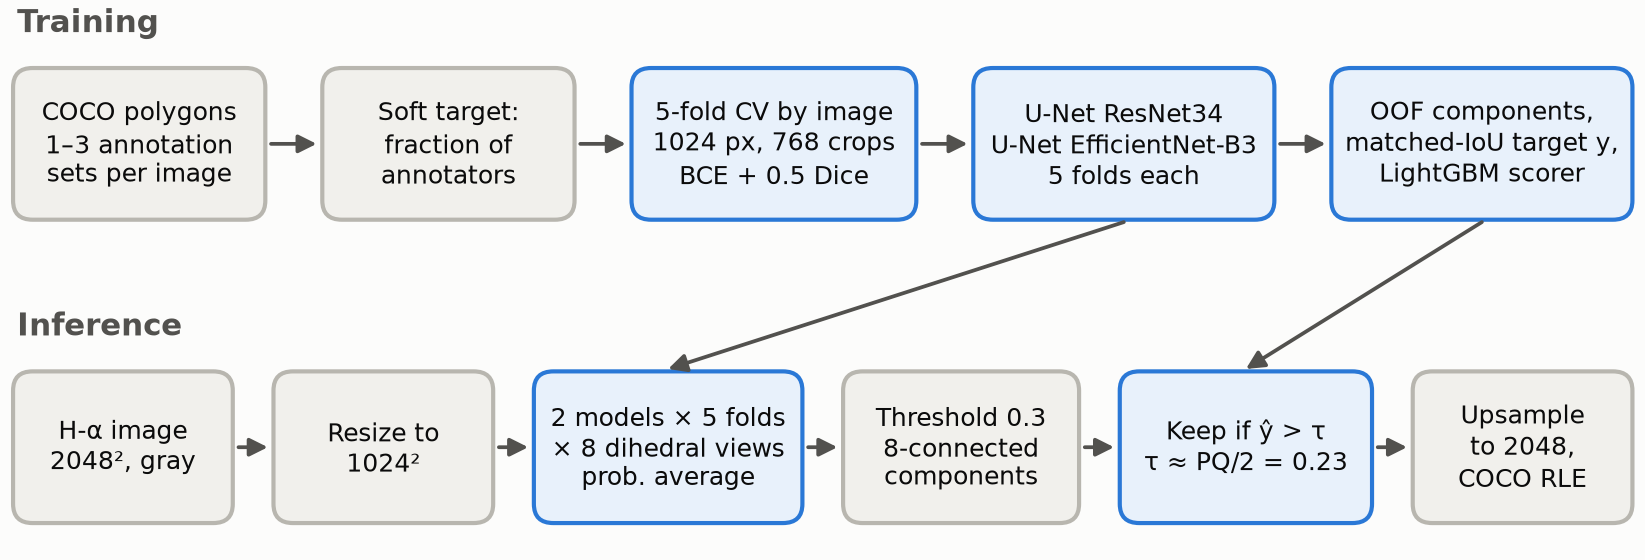
\includegraphics[width=0.92\textwidth]{fig_pipeline.png}
  \caption{End-to-end data pipeline. Blue boxes are learned components; arrows from the training row show where trained models enter inference.}
  \label{fig:pipeline}
\end{figure*}

\subsection{Metric analysis and keep rule}
    The host PQ loops over the annotation sets of each image; a predicted mask and a ground-truth mask form a true positive (TP) whenever their IoU exceeds 0.5, and counts are pooled over all sets:
    $\mathrm{PQ}=\sum_{TP}\mathrm{IoU}\,/\,(|TP|+\tfrac12|FP|+\tfrac12|FN|)$ \cite{kirillov2019panoptic}.
    We re-implemented it following the host's self-evaluation notebook; scoring each annotator against the others reproduces the publicly reported inter-annotator PQ of 0.340. Consider one predicted instance on an image with $n$ annotation sets that matches $k$ of them with IoUs $s_1,\dots,s_k$. Keeping it adds $\sum_j s_j$ to the numerator and exactly $n/2$ to the denominator ($k$ FNs become TPs: $+k-\frac{k}{2}$; the $n-k$ unmatched sets add $\frac{n-k}{2}$ FPs). Keeping it therefore raises PQ if and only if
    \begin{equation}
      y \equiv \frac{1}{n}\sum_{j=1}^{k} s_j \;>\; \frac{\mathrm{PQ}}{2}.
      \label{eq:keep}
    \end{equation}
    A real filament marked by only a minority of annotators should be dropped. This motivates every design choice below.

\subsection{Data, target and sampling}
    Images are used as single-channel grayscale. COCO polygons are rasterized per annotation set, and the training target is the per-pixel fraction of annotators that marked a filament (soft target). We use GroupKFold with five folds grouped by physical image, so annotation sets of one observation never straddle folds. All model selection, threshold tuning and scorer training use out-of-fold (OOF) predictions; no separate hold-out set is used, and the public leaderboard serves only as a sanity check. No external data is used; the public MAGFiLO release is excluded because it contains the test labels.

\subsection{Segmentation networks}
    We train U-Nets \cite{ronneberger2015unet} from \texttt{segmentation\_models\_pytorch} \cite{iakubovskii2019smp} with ImageNet-pretrained ResNet34 \cite{he2016resnet} and EfficientNet-B3 \cite{tan2019efficientnet} encoders. Images are resized to $1024\times1024$ (area interpolation) and training uses random $768\times768$ crops, dihedral augmentation (rotations by $90^\circ$, flips) and brightness, contrast and gamma jitter. The loss is BCE plus $0.5\times$ soft Dice; optimization uses AdamW with a OneCycle schedule (peak LR $5\times10^{-4}$), mixed precision, 30 epochs of 1200 crops, and batch size 4 (ResNet34) or 2 (EfficientNet-B3) to fit 4\,GB of VRAM.

\subsection{Inference and instance extraction}
    Each model predicts with 8-view dihedral test-time augmentation (TTA), and the five fold models of each architecture are averaged; the two architectures are then averaged with equal weights. The mean probability map is thresholded at 0.3 and split into 8-connected components, which gives disjoint instances by construction. Morphological post-processing (opening, closing, dilation) consistently reduced PQ and is not used.

\subsection{Instance scorer}
    For every OOF component we compute the target $y$ of Eq.~\eqref{eq:keep} against the ground truth and 24 features: area, bounding-box size, fill ratio and elongation; mean, maximum and standard deviation of probability and the fractions of pixels above 0.5, 0.7 and 0.9 (threshold persistence); the number of pieces the component splits into at threshold 0.6 (merge indicator); perimeter ratio and probability-edge sharpness; inner and surrounding-ring intensity and their contrast; distance to the solar-disk centre; image-level counts; and the per-model mean probabilities and their disagreement. A LightGBM regressor \cite{ke2017lightgbm} is trained fold-honestly (each fold scored by a model trained on the other four), and components with predicted $\hat y>\tau$ are kept. Per Eq.~\eqref{eq:keep}, the optimum should lie near PQ/2.

\subsection{Submission encoding}
    Selected components are mapped back to full resolution by re-thresholding the bilinearly upsampled $2048\times2048$ probability map and keeping each component that overlaps a selected one by more than 50\%. Masks are encoded as COCO run-length encoding (Fortran order). Every file is checked for empty masks, overlapping masks and orientation (RLE round-trip against ground truth).

\begin{figure*}[t]
  \centering
  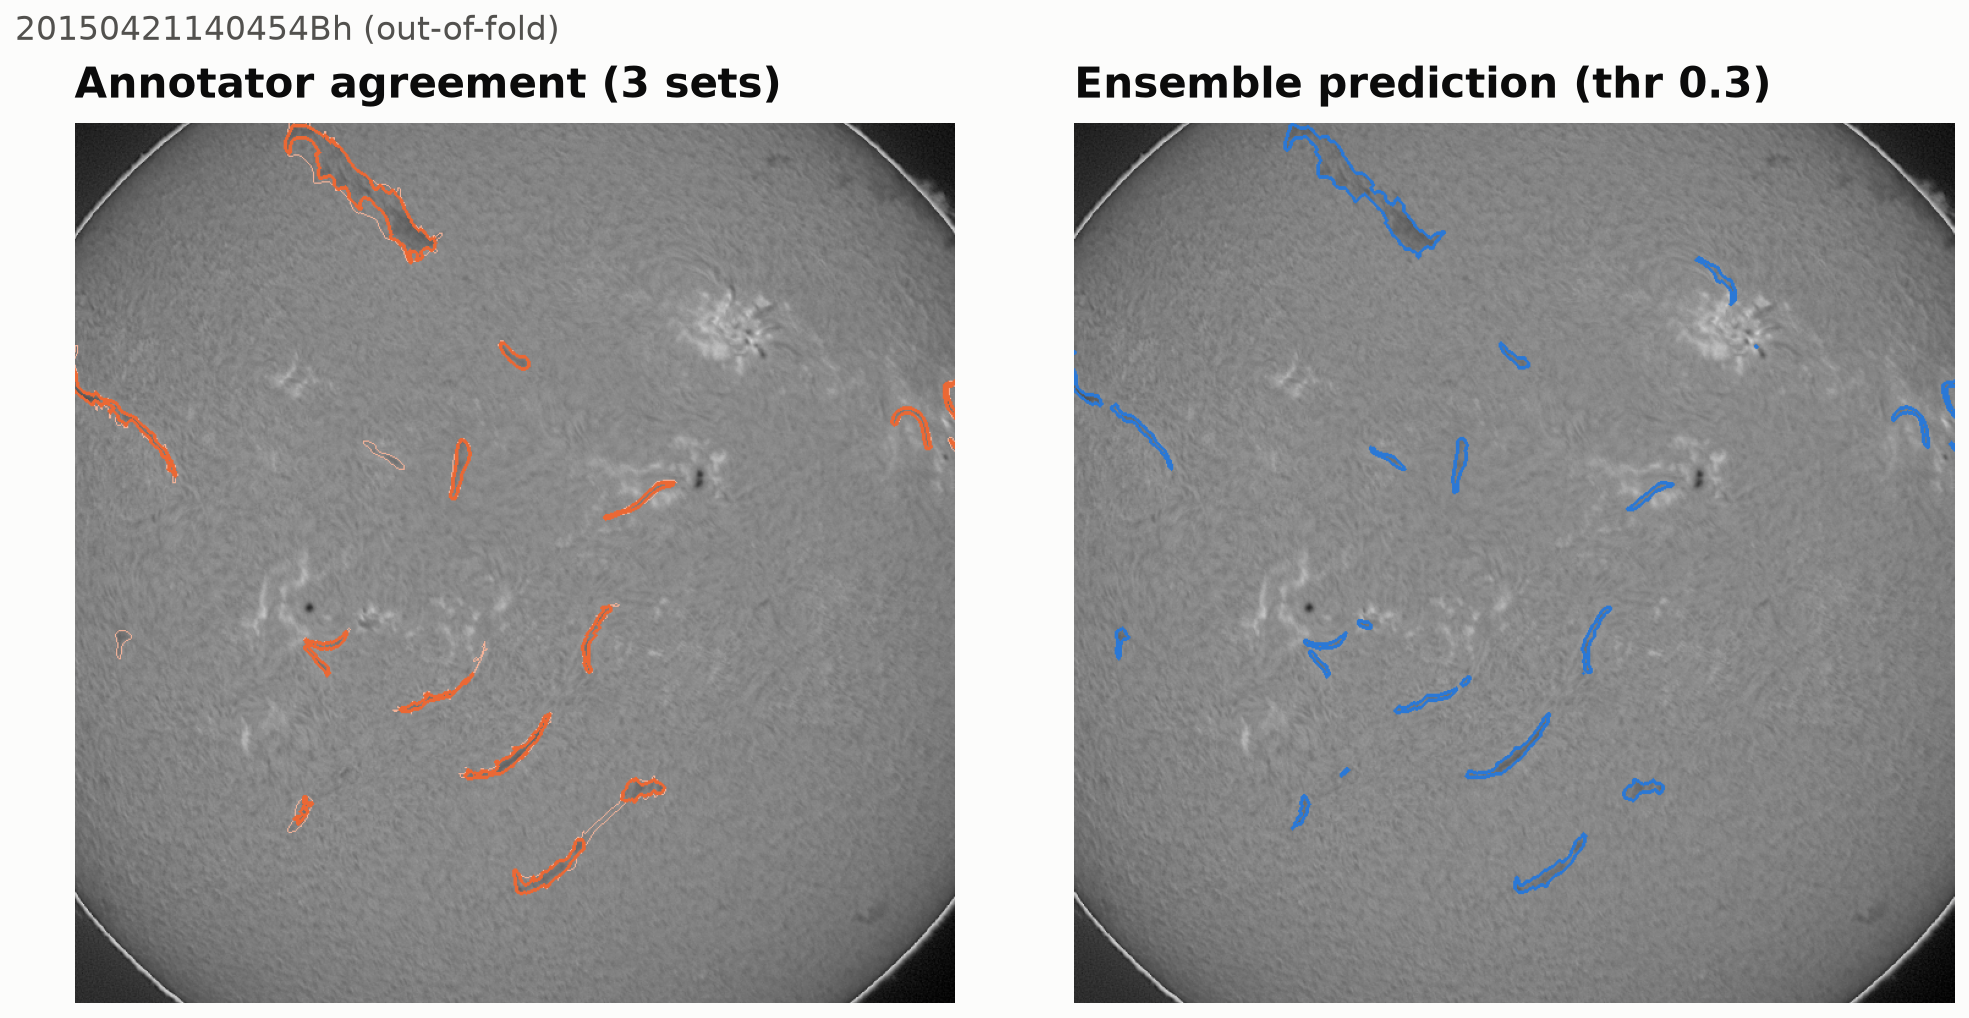
\includegraphics[width=0.86\textwidth]{fig_overlay.png}
  \caption{Out-of-fold example (3 annotation sets). Left: regions marked by at least 2 of 3 annotators (bold contours) and by a minority only (faint). Right: ensemble prediction. Majority filaments, including thin curved ones near active regions, are recovered as single contiguous instances; minority-only filaments are mostly, and deliberately, not predicted.}
  \label{fig:overlay}
\end{figure*}


% ==================================== %
%              EVALUATION              %
% ==================================== %
\section{Evaluation}\label{sec:evaluation}
\subsection{Strategy}
    We report pooled OOF PQ over all 1154 annotation sets, using our exact re-implementation of the host metric, with the standard deviation across the five folds as the uncertainty. Architectural choices were screened with single-change ablations on fold~0, with post-processing re-tuned for each variant, and then confirmed with full five-fold runs. As a reference for label noise, scoring each annotator against the other annotators of the same image gives PQ\,0.340.

\subsection{Results}
    Table~\ref{tab:results} summarizes the main configurations. CV ranking is preserved on the public leaderboard with a roughly constant offset of $-0.06$ to $-0.07$; the leaderboard uses about 90 images and two decimals, so it cannot resolve differences below $\approx$0.01.

\begin{table}[t]
  \caption{Grouped five-fold OOF PQ (mean $\pm$ fold std) and public leaderboard (LB).}
  \label{tab:results}
  \small
  \begin{tabular}{lcc}
    \toprule
    Configuration & CV PQ & LB\\
    \midrule
    R34, crop 512, components only & $0.386\pm0.007$ & 0.33\\
    R34, crop 512 + scorer & $0.401\pm0.011$ & 0.34\\
    R34, crop 768 + scorer & $0.424\pm0.008$ & 0.35\\
    R34 + EffB3 ensemble + scorer & $0.429\pm0.012$ & 0.35\\
    \quad + TTA8, extended scorer (final) & $\mathbf{0.432\pm0.011}$ & \textbf{0.36}\\
    \midrule
    Human vs.\ human & 0.340 & --\\
    \bottomrule
  \end{tabular}
\end{table}

    \textbf{Context beats resolution} (Fig.~\ref{fig:ablation}). Enlarging training crops from 512 to 768\,px adds $+0.031$ fold-0 PQ, and a full $1024\times1024$ input adds no more at twice the cost. Native $2048$ input with 640\,px crops (4$\times$ smaller field of view) loses $0.072$, while $1536$\,px input at the same field of view as 768@1024 gains nothing. Identifying a filament depends on large-scale context (limb, active regions, filament channels), not on finer pixels. A third ensemble member (UNet++ or a 1536\,px model) and 50 instead of 30 epochs each added $\le0.005$ and were dropped.

\begin{figure}[t]
  \centering
  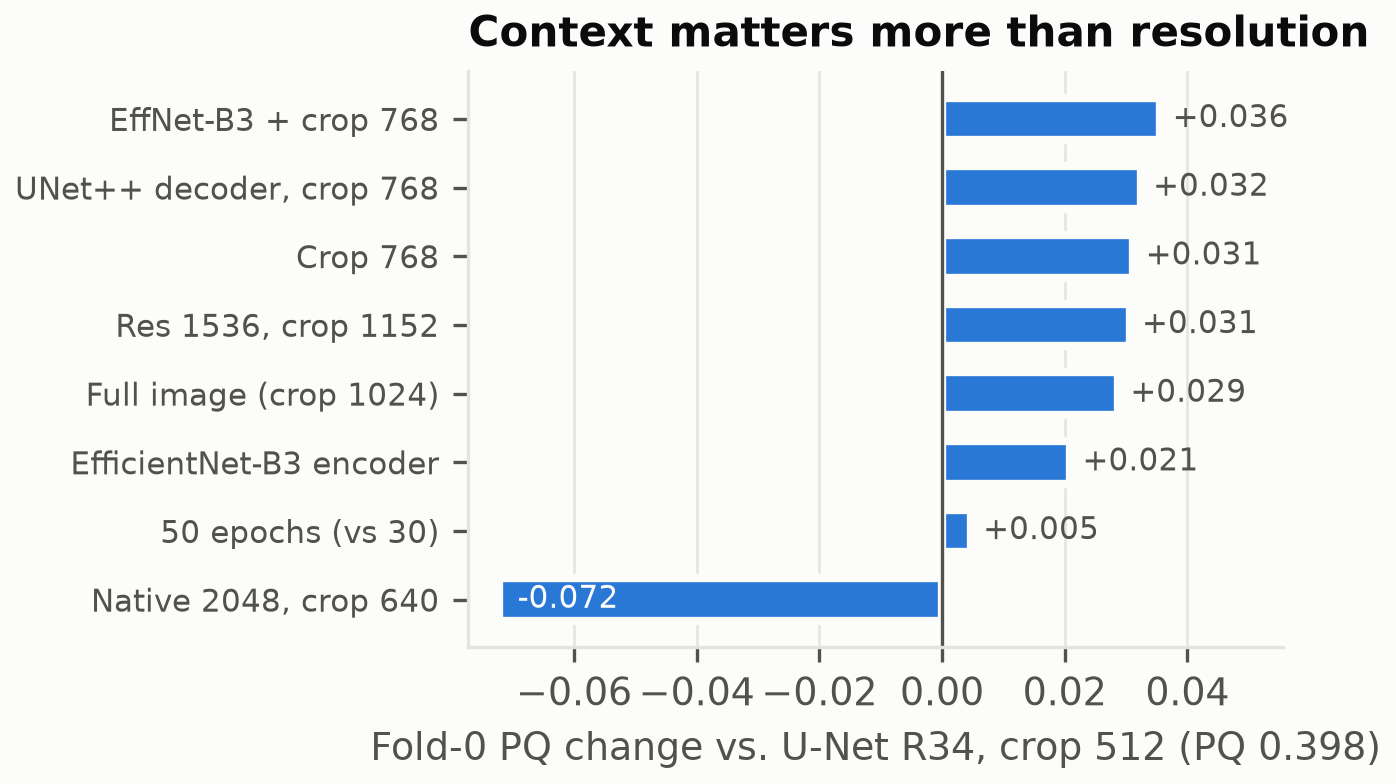
\includegraphics[width=\columnwidth]{fig_ablation.png}
  \caption{Single-change ablations on fold 0 (reference: R34, crop 512, PQ 0.398).}
  \label{fig:ablation}
\end{figure}

    \textbf{Instance scorer.} The scorer adds $+0.014$ to $+0.023$ PQ over the best area and probability filter on every model, and it improves every fold. The optimal threshold $\tau=0.23$ sits at PQ/2, as Eq.~\eqref{eq:keep} predicts (Fig.~\ref{fig:tau}).

\begin{figure}[t]
  \centering
  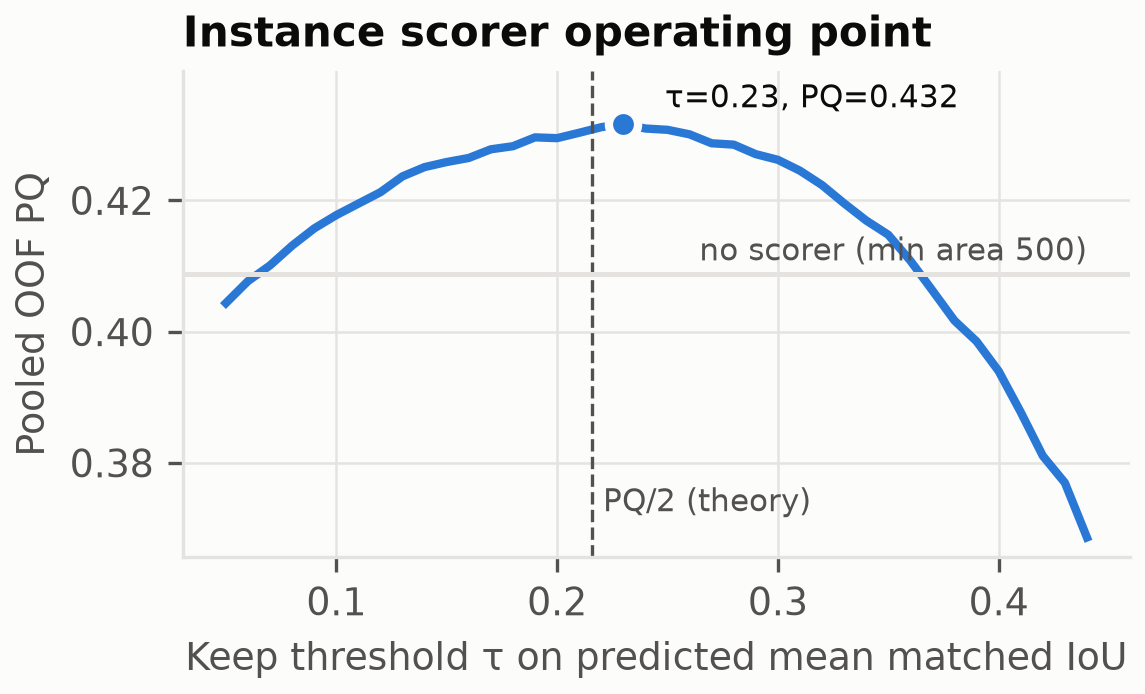
\includegraphics[width=\columnwidth]{fig_tau.png}
  \caption{Pooled OOF PQ of the final model vs.\ scorer keep threshold $\tau$; the dashed line marks PQ/2 from Eq.~\eqref{eq:keep}.}
  \label{fig:tau}
\end{figure}

\subsection{Error analysis, strengths and weaknesses}
    On fold~0 of the baseline, about half of the false negatives are filaments missed entirely, most of them small and marked by a minority of annotators. About a third of both FPs and FNs are near-misses with IoU 0.3--0.5, i.e.\ boundary disagreement of the same order as between annotators. Splits and merges cause fewer than 5\% of errors. Examples are shown in Fig.~\ref{fig:overlay}.

    \textit{Strengths.} The method is simple and fully reproducible on a 4\,GB GPU. Its instance selection is derived from the metric rather than tuned ad hoc, and it is stable across folds (std $\approx$0.01) and from CV to the leaderboard.

    \textit{Weaknesses.} By design, the method suppresses low-agreement filaments, so it under-reports faint or ambiguous structures that some annotators consider filaments. Fine barbs are smoothed at 1024\,px. Instances are connected components, so touching filaments can merge.

    \textit{Possible improvements.} Instance-aware heads (e.g.\ boundary or spine prediction) for touching filaments; a crop-level refinement network for boundaries; and per-annotator modeling of label noise instead of a single soft target. Our ablations indicate that these, rather than larger backbones or higher resolution, are where the remaining headroom lies.


% ==================================== %
%            ACKNOWLEDGMENT            %
% ==================================== %
\section{Acknowledgment}\label{sec:acknowledgment}
    % Do not change
    The organization of the Filament Segmentation Challenge 2026 is partially supported by the U.S. National Science Foundation (NSF) under Grant No. 2209912 and 2433781, directorate for Computer and Information Science and Engineering (CSE), and Office of Advanced Cyberinfrastructure (OAC), and Grant No. 2511630, AST Division Of Astronomical Sciences and MPS Directorate for Mathematical and Physical Sciences.

    The Filament Segmentation Challenge 2026 is sponsored by the U.S. National Science Foundation (NSF) National Solar Observatory (NSO).

    This work utilizes GONG data obtained by the NSO Integrated Synoptic Program, managed by the National Solar Observatory, which is operated by the Association of Universities for Research in Astronomy (AURA), Inc. under a cooperative agreement with the National Science Foundation and with contribution from the National Oceanic and Atmospheric Administration. The GONG network of instruments is hosted by the Big Bear Solar Observatory, High Altitude Observatory, Learmonth Solar Observatory, Udaipur Solar Observatory, Instituto de Astrofísica de Canarias, and Cerro Tololo Interamerican Observatory.

    We also thank the authors of public Kaggle notebooks whose ideas we re-implemented: soft annotator targets and instance keep thresholds (tushhaaarrrr), the evaluation metric (azimahmadzadeh), grouped cross-validation (dattadhebe), and operating-point selection (juanmirod).

\bibliographystyle{ACM-Reference-Format}
\bibliography{main}

\end{document}
